\chapter{Methodology and Implementation}
\label{cha:Chapter4_Methodology}

Length: 20-25 pages

Effort: 8 weeks+

Teilung zwischen Methodik (eher abstrakt) und Implementierung
Damit beginnen --> also mit Implementierung

Questions:
\begin{itemize}
\item Structure --> differentiation between getting the data, analysing the data and evaluating the results ok? --> Kann man machen
\item General idea: ``Readers should be able to carry out the same procedure using the thesis'' --> level of detail, e.g. cloud services? --> Implementierung auch auf Github zur Verfuegung stellen, API auf hoeherem Level (was machen die Funktionen verwenden),
Falls Cloud: nur virtueller Rechner --> eher nicht wichtig, falls spezifische Dienstleistung z.B. OpenAI (KI, Parsing) --> dann detaillierter, eher Richtung Implementation
\item Case study --> Evaluation of accuracy based on one real life topic? Topic, e.g. Covid-19 pandemic, german elections (aufpasssen, Politik schwer!), ...? --> je nach Umfang auch mehrere (sollen sich unterscheiden, Covid sehr viele Bereiche), Tweets auch auf Englisch
\end{itemize}

Content
\begin{itemize}
\item Data 
\begin{itemize}
    \item What data does twitter provide, auch z.B. Likes, Retweets
    \item Data extraction, Cloud Services --> spezifischer Dienst?
\end{itemize}
\item Analysis
\begin{itemize}
    \item Lexicon-Based Method
    \item Machine Learning Based Method
    \item Hybrid Method
\end{itemize}
\item Evaluation
\begin{itemize}
    \item Parameters --> objektive Kriterien, Qualitaet der Analyse Methode + Begruendung der Kriterien, Komplexitaet (Laufzeitkomplexitaet ja, Implementierung --> an sich nicht schlimm, aber robust? Abstuerze?)
    \item Case Study
    \item Qualitaet der Ergebnisse --> gut/schlecht, kann das akkurat erkannt werden?, evtl. menschliche Analyse, schoener: auf subjektive Einschaetzung verzichten
    \item Comparison with human tweets labeled by humans?
\end{itemize}
\end{itemize}


Analysis
\begin{itemize}
    \item Lexicon-Based Method
    \begin{itemize}
    \item General approach: Multiple lexicons with different topics, positive/neutral/negative
    \begin{itemize}
        \item Sentiment Words --> List of words with polarity, e.g. good
        \item Negation Words --> Words that negate the polarity of other words, e.g. not
        \item Intensity words --> Words that amplify the polarity, e.g. very
        \item Emoticons
    \end{itemize}
    \item Find the above word types in tweet
    \item Adjust polarity of sentiment words based on negation and/or intensity
    \item Calculate average of polarities including emoticons
    \item Example: The weather today is very terrible but the sound of rain is delightful.
    \begin{itemize}
        \item Sentiment of "very terrible": amplified negative (e.g. -2)
        \item Sentiment of "delightful": positive (e.g. +1)
        \item Overall: -2 + 1 = -1 --> negative
    \end{itemize}
    \item Comparison of different sentiment lexicons?
    \item Stop words --> needs, wants, etc. --> automatically negative (except for negation?)
    \item common idioms?
    \item slang
    \end{itemize}
    \item Machine Learning Based Method
    \begin{itemize}
        \item Naive Bayes --> probabilistic, multiple classes
        \begin{itemize}
            \item Based on Bayes theorem with conditional independence, add-one (laplace) smoothing, calculate P(x|y)
            \item Look at every word contained in tweet, apply formula to known words:
\[P(\mathrm{w}_{i}^{}|c) = \frac{count(\mathrm{w}_{i}^{}, c)+1}{(\sum_{w\in V}^{} (count(w,c)) + \left| V \right|} \]
            \item w = word, c is class (negative, positive), V is vocabulary of all known words
            \item Train with labelled tweets
           \[ \mathrm{c}_{NB}^{} = argmax_{c \in C}  P(c) \prod_{i \in positions}^{} P(\mathrm{w}_{i}^{}|c)\]
          
           
        \end{itemize}
        \item Logistic Regression? --> discriminative, binary classes
        \begin{itemize}
        \item Advantage: Not as many assumptions --> works better even when some features are correlated
        \end{itemize} 
        
    \end{itemize}
    \item Hybrid Method
    \begin{itemize}
        \item Approach 1 --> use lexicon-based score as an additional feature for the classifier (even if 0, it still can be classified)
        \item Combine the previous two or e.g. use a different classifier if that works better?
    \end{itemize}
\end{itemize}
\

New Learnings
\begin{itemize}
    \item Evaluation of different classifiers --> (J48), Naive Bayes (gaussian + multinominal distribution), Support Vector Machine, Logistic Regression, Random Forest
    \item Currently best: Naive Bayes with a multinomial distribution, 78.67\% of 4726 instances correct
    \item Caveats: Training for SVM and Logistic Regression not possible with all 1.2MM tweets --> system memory/runtime
    \item TODO: currently the ML method only recognized positive and neutral, more test instances?
    \item Lexicon Method: 75.68\% accurate on 9057 instances (includes neutral)
\end{itemize}

RandomForest
\begin{itemize}
    \item Collection of tree-structured classifiers
    \item Each tree depends on values of a random, independent vector
    \item Output is class selected by most trees
\end{itemize}

Questions
\begin{itemize}
    \item Fundamentals vs. Methodology: Wo z.B. Classifiers erklären?
    \item Welche Classifier wie vertiefen?
    \begin{itemize}
    \item Tabelle die Classifier vergleicht
    \item Kurze Erklärung aller Classifier?
    \item "Besten" Classifier tiefer erklären?
    \item z.B. Naive Bayes: Multinominale und Gaußsche Verteilung vergleichen/erklären?
    \end{itemize}
    \item Spezifische Bibliothek erwähnen (weka), Filter genauer (speichert nur 15000 Wörter, die mindestens 10x vorkommen, lowercase)?
    \item Daten beschreiben: Referenz + kurzer Überblick (Anzahl positiv/neutral/negativ, Themen, Zeitraum, bei Testdaten die Methode zur Klassifikation)
\end{itemize}

\section{Lexicon Method}
\TODO{TODO testen, paar Werte anpassen, stop words, etc.}


As previously mentioned, the lexicon method uses several dictionaries in order to classify a tweet. 


\TODO{preprocess, negation thing}


\begin{algorithm}[H]
  \caption{Lexicon algorithm}\label{euclid}
    \begin{algorithmic}[1]
        \Procedure{analyze}{$tweet$}\Comment{Sentiment score of tweet}
            \State $SentimentLexicon \gets$ Dictionary containing sentiment words with their polarities
            \State $NegationList \gets$ List containing negation words
            \State $IntensityLexicon \gets$ Dictionary containing intensity words with their multipliers
            \State $EmojiLexicon \gets$ Dictionary containing UTF-8 emojis with their polarities
            \ForEach {$word \in tweet$}
                \State $word \gets$ preprocess($word$)
                \State $score \gets 0.0$
                \If{$word \in SentimentLexicon$} 
                    \State $polarity \gets 1$
                    \For{\texttt{previous two words}}
                        \If{$previousWord \in NegationList$}
                            \State $polarity \gets polarity * (-1)$
                        \Else
                            \If{$previousWord \in IntensityLexicon$}
                                \State $polarity \gets polarity * intensity$
                            \EndIf
                        \EndIf
                    \EndFor
                    \State $score \gets score + polarity * sentiment$
                \Else
                    \If{$word \in EmojiLexicon$}
                        \State $score \gets score + emojiSentiment$
                    \EndIf
                \EndIf 
            \EndFor
            \State \textbf{return} $score$
        \EndProcedure
    \end{algorithmic}
\end{algorithm}




\section{Machine Learning Method}
    \subsection{Naive Bayes}
        Naive Bayes is a probabilistic classification model. It is based on the Bayes theorem, which is shown in Equation \eqref{eq:bayes}:
        \begin{equation}
            \label{eq:bayes}
            P(c_j|d_i) = \frac{P(c_j) * P(d_i|c_j)}{P(d_i)}
        \end{equation}
        where $c$ is the class label and $d$ is a set of attribute values \cite{DBLP:books/aw/TanSKK2019}. 
        
        \TODO{Zitat abändern}

        Bayes theorem allows to calculate the posterior probability $P(c|d)$, which Tan et al. describe as "the probability of observing a class label $c$ for a data instance given its set of attribute values $d$" \cite[p.~418]{DBLP:books/aw/TanSKK2019}. 

        To calculate the posterior probability, the class conditional probability $P(d|c)$ is needed, which describes the probability of observing a set of attribute values given a class. One approach to calculate the class conditional probability outlined by Tan et al. is to ''consider the fraction of training instances of a given class for every possible combination of attribute values'' \cite[p.~419]{DBLP:books/aw/TanSKK2019}. With a large number of attributes and values, this method becomes computationally infeasible due to the exponential growth of combinations \cite{DBLP:books/aw/TanSKK2019}.

        Due to this, the Naive Bayes assumption is employed to estimate the class conditional probability. Naive Bayes uses conditional independence, which states that attribute values are only dependent on the class label and not each other. Thus, the class conditional probability can be calculated by using Equation \eqref{eq:naive_assumption}:
        \begin{equation}
            \label{eq:naive_assumption}
            P(d_i|c_j) = \prod_{t=1}^{n}P(w_{t}|c_j)
        \end{equation}
        with $d_i$ containing $n$ attributes $\{w_1,w_2,...,w_t\}$ \cite{DBLP:books/aw/TanSKK2019}.

        Furthermore, $P(d)$ remains constant for every class label $c$, so the class that maximizes Equation \eqref{eq:naive_final} is chosen: 
        \begin{equation}
            \label{eq:naive_final}
            P(c_j|d_i)\propto P(c_j)\prod_{t=1}^{n}P(w_{t}|c_j) 
        \end{equation}   
        
        \TODO{P(c) eingehen}
        
        There are different models on how to implement the Naive Bayes assumption for text classification. McCallum and Nigan compared two models, a multivariate Bernoulli model, and a multinomial model. \TODO{multi-variate, aber wie genau?}
        
        According to McCallum and Nigan, "the multinomial model captures word frequency information in documents" \cite[p.~3]{Mccallum1998}. In this case, a document is represented by a tweet. By considering not only if a word is present but also how often it is present, the Bernoulli model's restriction to two values becomes uninformative. They describe the document as being "an ordered sequence of word events, drawn from the same vocabulary V" \cite[p.~3]{Mccallum1998}, with its length being independent of class. Using Naive Bayes, we assume that every word event is independent.
        
        \TODO {weg? oder Gleichung?}
        
        According to Forbes et al., "the multinomial variate is a multidimensional generalization of the binomial. Consider a trial that can result in only one of $k$ possible distinct outcomes, labeled $A_i, i = 1,...,k$. The outcome $A_i$ occurs with probability $p_i$. The multinomial distribution relates to a set of n-independent trials of this type." \cite[p.~135]{evans2011statistical}.
        
        Applying this to the model, McCallum and Nigan state that "each document $d_i$ is drawn from a multinomial distribution of words with as many independent trials as the length of $d_i$" \cite[p.~3]{Mccallum1998}. Using the multinomial distribution, the class conditional probability can then be calculated using Equation \eqref{eq:multinomial_bayes}:
        \begin{equation}
            \label{eq:multinomial_bayes}
                P(d_i|c_j) = P(|d_i|)|d_i|!\prod_{t=1}^{|V|}\frac{P(w_t|c_j)^{N_{i_t}}}{N_{i_t}!}
        \end{equation}
        
        with the document $d_i$ containing $|V|$ words $w_t$, $N_{i_t}$ being the number of times $w_t$ appears in $d_i$ and $c_j$ describing a class \cite{Mccallum1998}. 
        
        To estimate $P(w_t|c_j$, the probability of a word $w_t$ given a class $c_j$, training instances are used to count the number of times a word appears in a class in Equation \eqref{eq:prob_word}:
        \begin{equation}
            \label{eq:prob_word}
                P(w_t|c_j) = \frac{1 + \sum_{i=1}^{|D|}N_{it} + P(c_j|d_i)}{|V| + \sum_{s=1}^{|V|} \sum_{i=1}^{|D|}N_{is} P (c_j|d_i)} 
        \end{equation}
        with $D$ containing labeled training documents $d_i$, $N_{it}$ describing the number of times $w_t$ appears in document $d_i$ and $|V|$ containing all words.
        Because the class conditional probabilities for labeled instances is 1 for one instance, and 0 for the other ones, Equation \eqref{eq:prob_word} can be simplified into Equation \eqref{eq:prob_word_simpler}:
                \begin{equation}
            \label{eq:prob_word_simpler}
                P(w_t|c_j) = \frac{1 + N_{tj}}{|V| + \sum_{s=1}^{|V|}N_{sj}} 
        \end{equation}
        \TODO{evtl. anderes N, erklaeren, etc.}
        
        
        with $N_{tj}$ being the number of training instances in class $c_j$ containing the word $w_t$. 
        
        By using Equation \eqref{eq:prob_word}, we calculate the word probability $P(w_t|c_j$). We utilize this in Equation \eqref{eq:multinomial_bayes} to calculate the class conditional probability $P(d_i|c_j)$ using the multinomial distribution. Finally, this allows us to estimate the posterior probability $P(c|d)$, as shown in Equation \eqref{eq:naive_final}. By selecting the class with the higher posterior probability, the classifier is able to make a prediction.
        
\subsection{Random Forest}
        According to Tan et al., Random Forest is an ensemble method that utilizes multiple base classifiers to take a vote on their predictions. The final prediction is then made by either averaging the vote or taking the majority vote. Random Forest applies a set of decorrelated decision trees by implementing two key characteristics.
        
        The first characteristic is Bagging. Each tree is trained by a data set that was sampled from the original training data. Because the sampling is done with replacement and the samples must have the same size as the original training data, the sample will, on average, only contain 63\% of the original data.
        
        The selection of input attributes is the second characteristic. When a tree is being constructed, an attribute must be selected for splitting at each internal node.
        Random Forest randomly chooses a subset of attributes, from which the attribute with the maximum reduction in an impurity measure is chosen.
        
        Through these characteristics, Random Forest reduces the correlation of trees and thus the variance \cite{DBLP:books/aw/TanSKK2019}.
        
        \begin{figure}[h!]
        \centering
        \begin{tikzpicture}
        [
        grow                    = right,
    sibling distance        = 4em,
    level distance          = 9em,
    edge from parent/.style = {draw, -latex},
    every node/.style       = {font=\footnotesize},
    sloped
  ]
  \node [root] {}
    child { node [dummy] {}
      child { node [dummy] {}
        child { node [dummy] {}
            child { node [env] {$-1.0$}
                edge from parent node [below, align=center] {$studying < 0.5$} }
            child { node [env] {$+1.0$}
                edge from parent node [above] {$studying \geq 0.5$} }
            edge from parent node [below] {$will < 0.5$} }
        child { node [env] {$-1.0$}
                edge from parent node [above] {$will \geq 0.5$} }
        edge from parent node [below] {$hates < 0.5$} }
      child { node [env] {$-1.0$}
              edge from parent node [above, align=center]
                {$hates \geq 0.5$}}
              edge from parent node [above] {$hurts \geq 0.5$} };
\end{tikzpicture}
    \caption{Part of a tree generated by the Random Forest classifier.}
      \label{fig:tree}
\end{figure}
\TODO{satzzeichen nach Gleichung, siehe Buch}
\TODO{citations}
\subsection{Logistic Regression}
Logistic Regression calculates the posterior probability $P(c_j|d_i)$ directly, without relying on the class conditional probability such as Naive Bayes, which is why it is a probabilistic discriminative model. In a binary model, the class label can be assigned by calculating the odds, as seen in Equation \eqref{eq:logistic_odds}:
        \begin{equation}
            \label{eq:logistic_odds}
                \frac{P(c=1|d)}{P(c=0|d)}
        \end{equation}
If the odds are greater than 1, then the class label 1 can be assigned to document d, otherwise class 0 is assigned. Logistic Regression represents the odds using a linear predictor $z=w^Tx + b$, which results in equation \eqref{eq:logistic_linear}:
        \begin{equation}
            \label{eq:logistic_linear}
                \frac{P(c=1|d)}{P(c=0|d)} = e^z = e^{w^Td+b}
        \end{equation}
with the parameters $w$ and $b$ and $w^t$ signifying the vector transpose \cite{DBLP:books/aw/TanSKK2019}.

By substituting $P(c=0|d)$ with $1 - P(c=1|x)$ and solving for $P(c=1|d)$, we get Equation \eqref{eq:logistic_sigmoid}:
        {\begin{equation}
            \label{eq:logistic_sigmoid}
                P(c=1|d) = \frac{1}{1+e^{-z}} = \sigma(z)
        \end{equation}}
$\sigma(z)$ is called the sigmoid function, whose graph can be seen in Figure \ref{fig:sigmoid}:
        \begin{figure}[h!]
        \centering

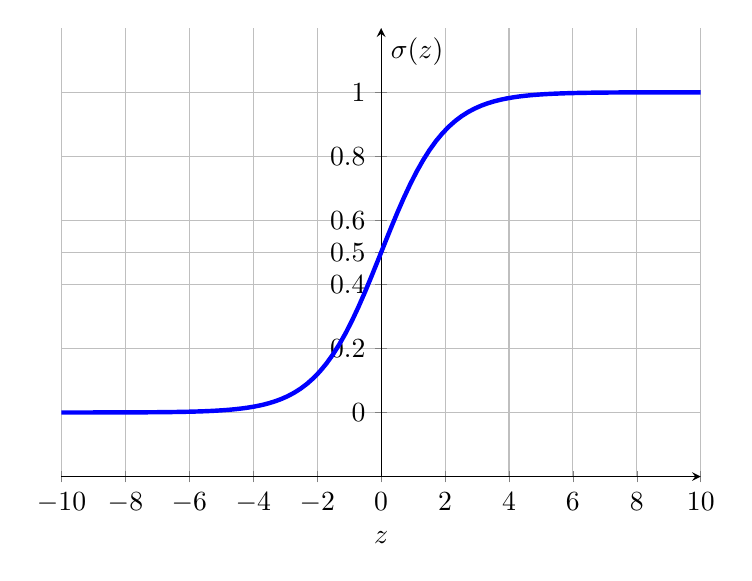
\begin{tikzpicture}
\begin{axis}
[
    grid=major,   
    xmin=-10,
    xmax=10,
    axis x line=bottom,
    ytick={0,.2,.4,.5,.6,.8,1},
    ymax=1.2,
    ymin=-0.2,
    axis y line=middle,
    width=0.8\textwidth,
    height=0.6\textwidth,
    xlabel={$z$},
    ylabel={$\sigma(z)$}
]
    \addplot%
    [
        blue,%
        mark=none,
        samples=100,
        domain=-10:10,
        ultra thick
    ]
    (x,{1/(1+exp(-x))});
\end{axis}
\end{tikzpicture}
    \caption{Plot of sigmoid function $\sigma(z)$.}
      \label{fig:sigmoid}
\end{figure}

As seen in Figure \ref{fig:sigmoid}, $\sigma(z) \geq 0.5$ when $z \geq 0$, so if $z \geq 0$, we assign the instance $d_i$ to the class $c = 1$.

Using training instances, the parameters $w$ and $b$ can be learned and thus the posterior probability $P(c_j|d_i)$ can be estimated \cite{DBLP:books/aw/TanSKK2019}.

\subsection{Support Vector Machine}



    

        
    
        
        
\section{Evaluation}
\begin{table}[h!]
\centering
\caption{Table to test captions and labels.}
\begin{tabular}{ |p{3cm}||p{3cm}|p{2cm}|p{2cm}|p{2cm}|p{2cm}|  }
 \hline
 Classifier name &          Parameters &             Training Instances &    Accuracy &      Kappa &     Relative absolute error \\
 \hline
 Naive Bayes (Gauss)        &-&            TODO&                 60.99\%&        0.21&       82.14\%\\
  \hline
 Naive Bayes (Multinomial)  &-&                     1231862&                78.67\%&        0.51&       52.22\%\\
  \hline
 Random Forest              &depth = 300&            12318&                 75.48\%&        0.45&       81.33\%\\
  \hline
 Logistic Regression        &iterations = 10&            94655&                 77.40\%&        0.47&       59.70\%\\
  \hline
 Support Vector Machine     &kernel = linear&            TODO&                 77.11\%&        0.48&       45.52\%\\
 \hline
\end{tabular}
\label{tab:evaluations}
\end{table}












